% ==========================================
% CAPÍTULO 3: DESARROLLO / RESULTADOS Y PRUEBAS
% ==========================================


% ==========================================
% INSTRUCCIONES GENERALES PARA ESTE CAPÍTULO:
% ==========================================
% 1. Se recomienda escribir con propias palabras (el profe lo aprecia).
% 2. Se sugiere ser específico: podrías mencionar qué funciones de MPI usaste y POR QUÉ.
% 3. Sería conveniente explicar el FLUJO de tu programa paso a paso.
% 4. Incluir fragmentos de código, pero solo los más relevantes.
% 5. Se sugiere que las capturas de pantalla sean claras y legibles.
% ==========================================

% Responsable: Luna.

\chapter{Resultados y pruebas}
% Ejemplo: "En este capítulo se presenta el desarrollo del sistema de...
%           Se detalla el diseño del código fuente, las funciones MPI
%           utilizadas y la evidencia de ejecución en el cluster."

En este capítulo se presenta el desarrollo integral del sistema de procesamiento paralelo basado en la interfaz de paso de mensajes (MPI). Se detallará la lógica implementada en el código fuente escrito en el lenguaje C, se explicarán minuciosamente las funciones de MPI seleccionadas para la coordinación de tareas y, finalmente, se mostrará la evidencia gráfica de la ejecución del programa, garantizando que el flujo de datos opere correctamente bajo un esquema concurrente \cite{ref2_frem}.

\section{Desarrollo del Sistema}

% ==========================================
% SUGERENCIAS
% ==========================================
% 1. Podrías explicar el PROBLEMA que resuelve tu programa.
%    - ¿Qué cálculo realiza? (ej. suma de vectores, multiplicación de matrices,
%      aproximación de pi, ordenamiento paralelo, etc.)
%    - ¿Por qué es adecuado resolverlo con MPI?
%
% 2. Se sugiere describir la ESTRATEGIA DE PARALELIZACIÓN.
%    - ¿Cómo dividiste el trabajo entre los procesos? (división de dominio,
%      división de tareas, maestro-trabajador, etc.)
%    - ¿Cuántos procesos usaste y por qué?
%
% 3. Opcionalmente, podrías mencionar las FUNCIONES MPI CLAVE que utilizaste.
%    - Ejemplos: MPI_Init, MPI_Comm_size, MPI_Comm_rank, MPI_Send, MPI_Recv,
%      MPI_Bcast, MPI_Scatter, MPI_Gather, MPI_Reduce, MPI_Finalize, etc.
%    - Se recomienda no solo listarlas, sino explicar PARA QUÉ las usaste en el programa.
%
% 4. Diagrama de flujo (completamente opcional).
%    - Si lo deseas, podrías incluir un diagrama simple del flujo de comunicación entre procesos.
%    - Quizás guardes la imagen en imagenes/ e la insertes con \includegraphics.
% ==========================================

Para dar solución al requerimiento de procesamiento de datos, el problema central consistió en procesar múltiples operaciones aritméticas de forma concurrente, cada una dependiente de un conjunto específico de valores flotantes (a, b y c). En lugar de calcular cada operación de manera secuencial, lo cual subutiliza los recursos de hardware, resulta mucho más adecuado abordar este problema empleando MPI. Esta tecnología permite instanciar múltiples procesos de trabajo independientes que pueden ejecutar sus cálculos matemáticos al mismo tiempo, lo que acelera significativamente la obtención de resultados globales.

La estrategia de paralelización adoptada fue un esquema de maestro-trabajador mediante la división de tareas \cite{ref4_frem}. Para este fin, se emplearon exactamente ocho procesos, ya que la carga de trabajo estipula la evaluación de siete operaciones distintas, requiriendo un proceso adicional que actúe como nodo principal. Las responsabilidades se dividieron de forma jerárquica para optimizar la distribución de flujos de datos a través de la red de interconexión. Por un lado, el Proceso 0, o nodo maestro, contiene la matriz de datos completa, la distribuye fila por fila a los demás nodos, y finalmente recolecta los resultados para imprimirlos de forma ordenada. Por otro lado, los Procesos del 1 al 7 fungen como trabajadores, encargándose cada uno de recibir su respectiva carga de trabajo, ejecutar una fórmula matemática única con dichos valores de entrada y retornar el conjunto de variables ya computado directamente de vuelta al procesador maestro. 

Durante el desarrollo del sistema se emplearon diversas rutinas clave de la biblioteca MPI, cuyo uso fue de carácter fundamental para el acoplamiento de los procesos. En primera instancia, la función \texttt{MPI\_Init} fue utilizada estrictamente para levantar e inicializar el entorno de ejecución paralelo maestro mucho antes de proceder con cualquier manipulación de la red de área local. Seguidamente, las rutinas de interrogación de \texttt{MPI\_Comm\_rank} y \texttt{MPI\_Comm\_size} fueron invocadas de manera complementaria para poder obtener el identificador numérico (rango) particular de cada proceso y validar así que, bajo cualquier circunstancia, se cuente con la presencia activa de los ocho nodos elementales que sostienen el diseño lógico. Por último, la estructura de comunicación se implementó con \texttt{MPI\_Send} y \texttt{MPI\_Recv}, mediante intercambios punto a punto. Gracias a ello, el nodo maestro distribuyó de forma ordenada los arreglos numéricos junto con un \textit{token} de sincronización, y después recibió de cada proceso trabajador el resultado aritmético correspondiente \cite{ref7_frem}.

% TIP: Si tu práctica tiene varios ejercicios, podrías crear una subsección para cada uno:
%      \subsection{Ejercicio 1: Suma de vectores}
%      \subsection{Ejercicio 2: Producto punto}

\section{Diseño y Código Fuente}

% ==========================================
% SUGERENCIAS
% ==========================================
% 1. Se sugiere presentar los FRAGMENTOS DE CÓDIGO MÁS IMPORTANTES.
%    - Podrías seleccionar las partes clave.
%    - Ejemplos de fragmentos útiles:
%      * Inicialización de MPI y obtención del rank/size.
%      * Distribución de datos (Scatter/Broadcast).
%      * Cálculo principal en cada proceso.
%      * Recolección de resultados (Gather/Reduce).
%
% 2. Se recomienda usar el entorno `lstlisting` PARA CÓDIGO.
%    Ejemplo:
%    \begin{lstlisting}[language=C++, caption=Inicializacion MPI]
%    int rank, size;
%    MPI_Init(&argc, &argv);
%    MPI_Comm_rank(MPI_COMM_WORLD, &rank);
%    MPI_Comm_size(MPI_COMM_WORLD, &size);
%    \end{lstlisting}
%
% 3. Podrías comentar cada fragmento de código con tu propia explicación.
%    - ¿Qué hace esta parte del código?
%    - ¿Por qué es importante para la paralelización?
%
% 4. Se sugiere explicar el ALGORITMO detalladamente.
%    - Pseudocódigo o descripción paso a paso.
%    - Complejidad computacional (si aplica).
% ==========================================

% TIP: Si el código es muy largo, coloca la versión completa en el APÉNDICE
%      y aquí solo pon los fragmentos más relevantes con explicación.

% TIP: La plantilla ya incluye el paquete `listings` configurado.
%      Si necesitas resaltar sintaxis de C/C++, usa:
%      \begin{lstlisting}[language=C++, caption=Titulo del codigo]

El núcleo algorítmico del proyecto se apoya en un control estricto de la comunicación. A continuación, se explican paso a paso los fragmentos más relevantes involucrados en este proceso. En primera instancia, el archivo de configuración \texttt{Makefile} establece las reglas para la compilación del proyecto utilizando el compilador \texttt{mpicc}, garantizando un nivel alto de revisión mediante las banderas \texttt{-Wall} y \texttt{-Wextra}. La inclusión de este generador automatiza estructuralmente la creación del binario ejecutable final, a la vez que abstrae considerablemente el desgaste operativo que implicaría la invocación rutinaria y manual de todas las pruebas. Para garantizar verdaderamente su reproducibilidad en multiplicidad de entornos o ecosistemas afines a GNU Linux, esta distribución documental expone formalmente sus directrices sintácticas constitutivas. Por lo tanto, en la Figura \ref{fig:codigo_makefile} se muestra la visualización completa del archivo \texttt{Makefile}.

\begin{figure}[htbp]
\centering
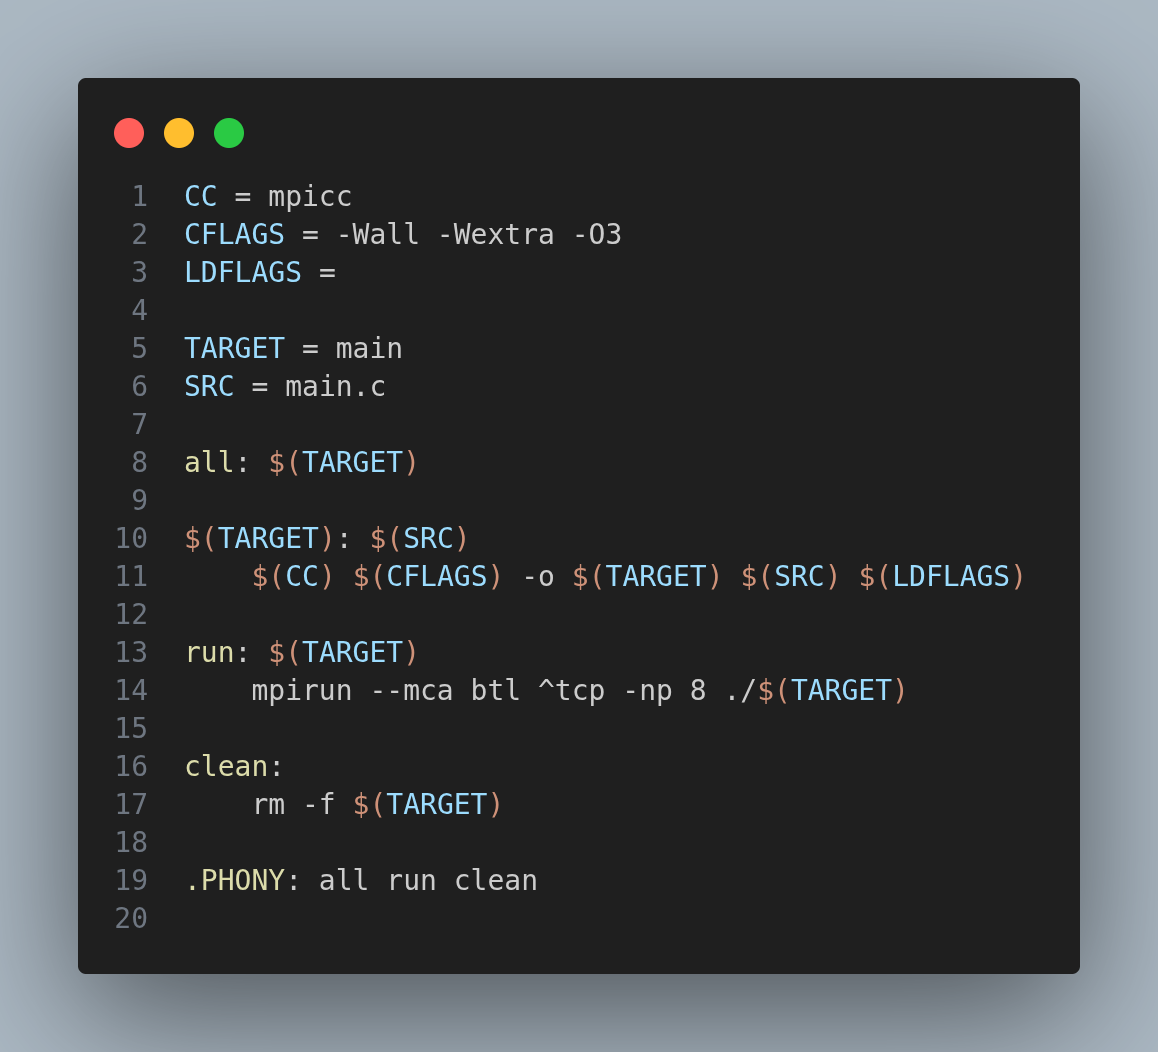
\includegraphics[width=0.8\textwidth]{imagenes/Hako/codigo_makefile.png}
\caption{Archivo de configuración Makefile. Fuente: Elaboración propia.}
\label{fig:codigo_makefile}
\end{figure}

Por otra parte, el archivo principal \texttt{main.c}, cuyo contenido completo se incluye en el Anexo~\ref{chap:codigos_completos}, constituye el núcleo operativo del sistema paralelo, pues en él se definen tanto la estructura de datos compartida como la lógica de comunicación entre el nodo maestro y los siete trabajadores. Al inicio del programa se incluyen las bibliotecas estándar de C junto con \texttt{<mpi.h>}, se establece la constante \texttt{N\_COLUMNAS} con valor 3 y se declaran las variables que gestionarán los identificadores de proceso, los contenedores de mensajes y el estado de las operaciones \cite{ref7_frem}. Estas declaraciones preparan el terreno para que cada proceso, independientemente de su rol posterior, disponga de un espacio de memoria local donde almacenar temporalmente los valores recibidos y los resultados calculados.

Inmediatamente después de las declaraciones, se inicializa el entorno MPI mediante \texttt{MPI\_Init}, obteniéndose el rango del proceso con \texttt{MPI\_Comm\_rank} y el tamaño total del comunicador con \texttt{MPI\_Comm\_size}. Esta etapa es crítica porque cualquier desajuste en el número de procesos comprometería el reparto de trabajo estipulado; por ello, el programa verifica que \texttt{procesos} sea exactamente 8, de lo contrario el nodo 0 imprime un mensaje de error y se invoca \texttt{MPI\_Finalize} para cerrar el entorno de forma controlada. En la Figura~\ref{fig:codigo_main_1_sup} se observa esta primera mitad del código, donde quedan expuestas las directivas de preprocesador, la matriz de datos con los valores $(a,b,c)$ asignados a cada trabajador y la validación inicial que garantiza la integridad del despliegue.

% --- CÓDIGO MAIN 1: PARTE SUPERIOR (inicialización y validación) ---
\begin{figure}[H]
    \centering
    \adjustbox{trim=0 {0.47\height} 0 0, clip}{
        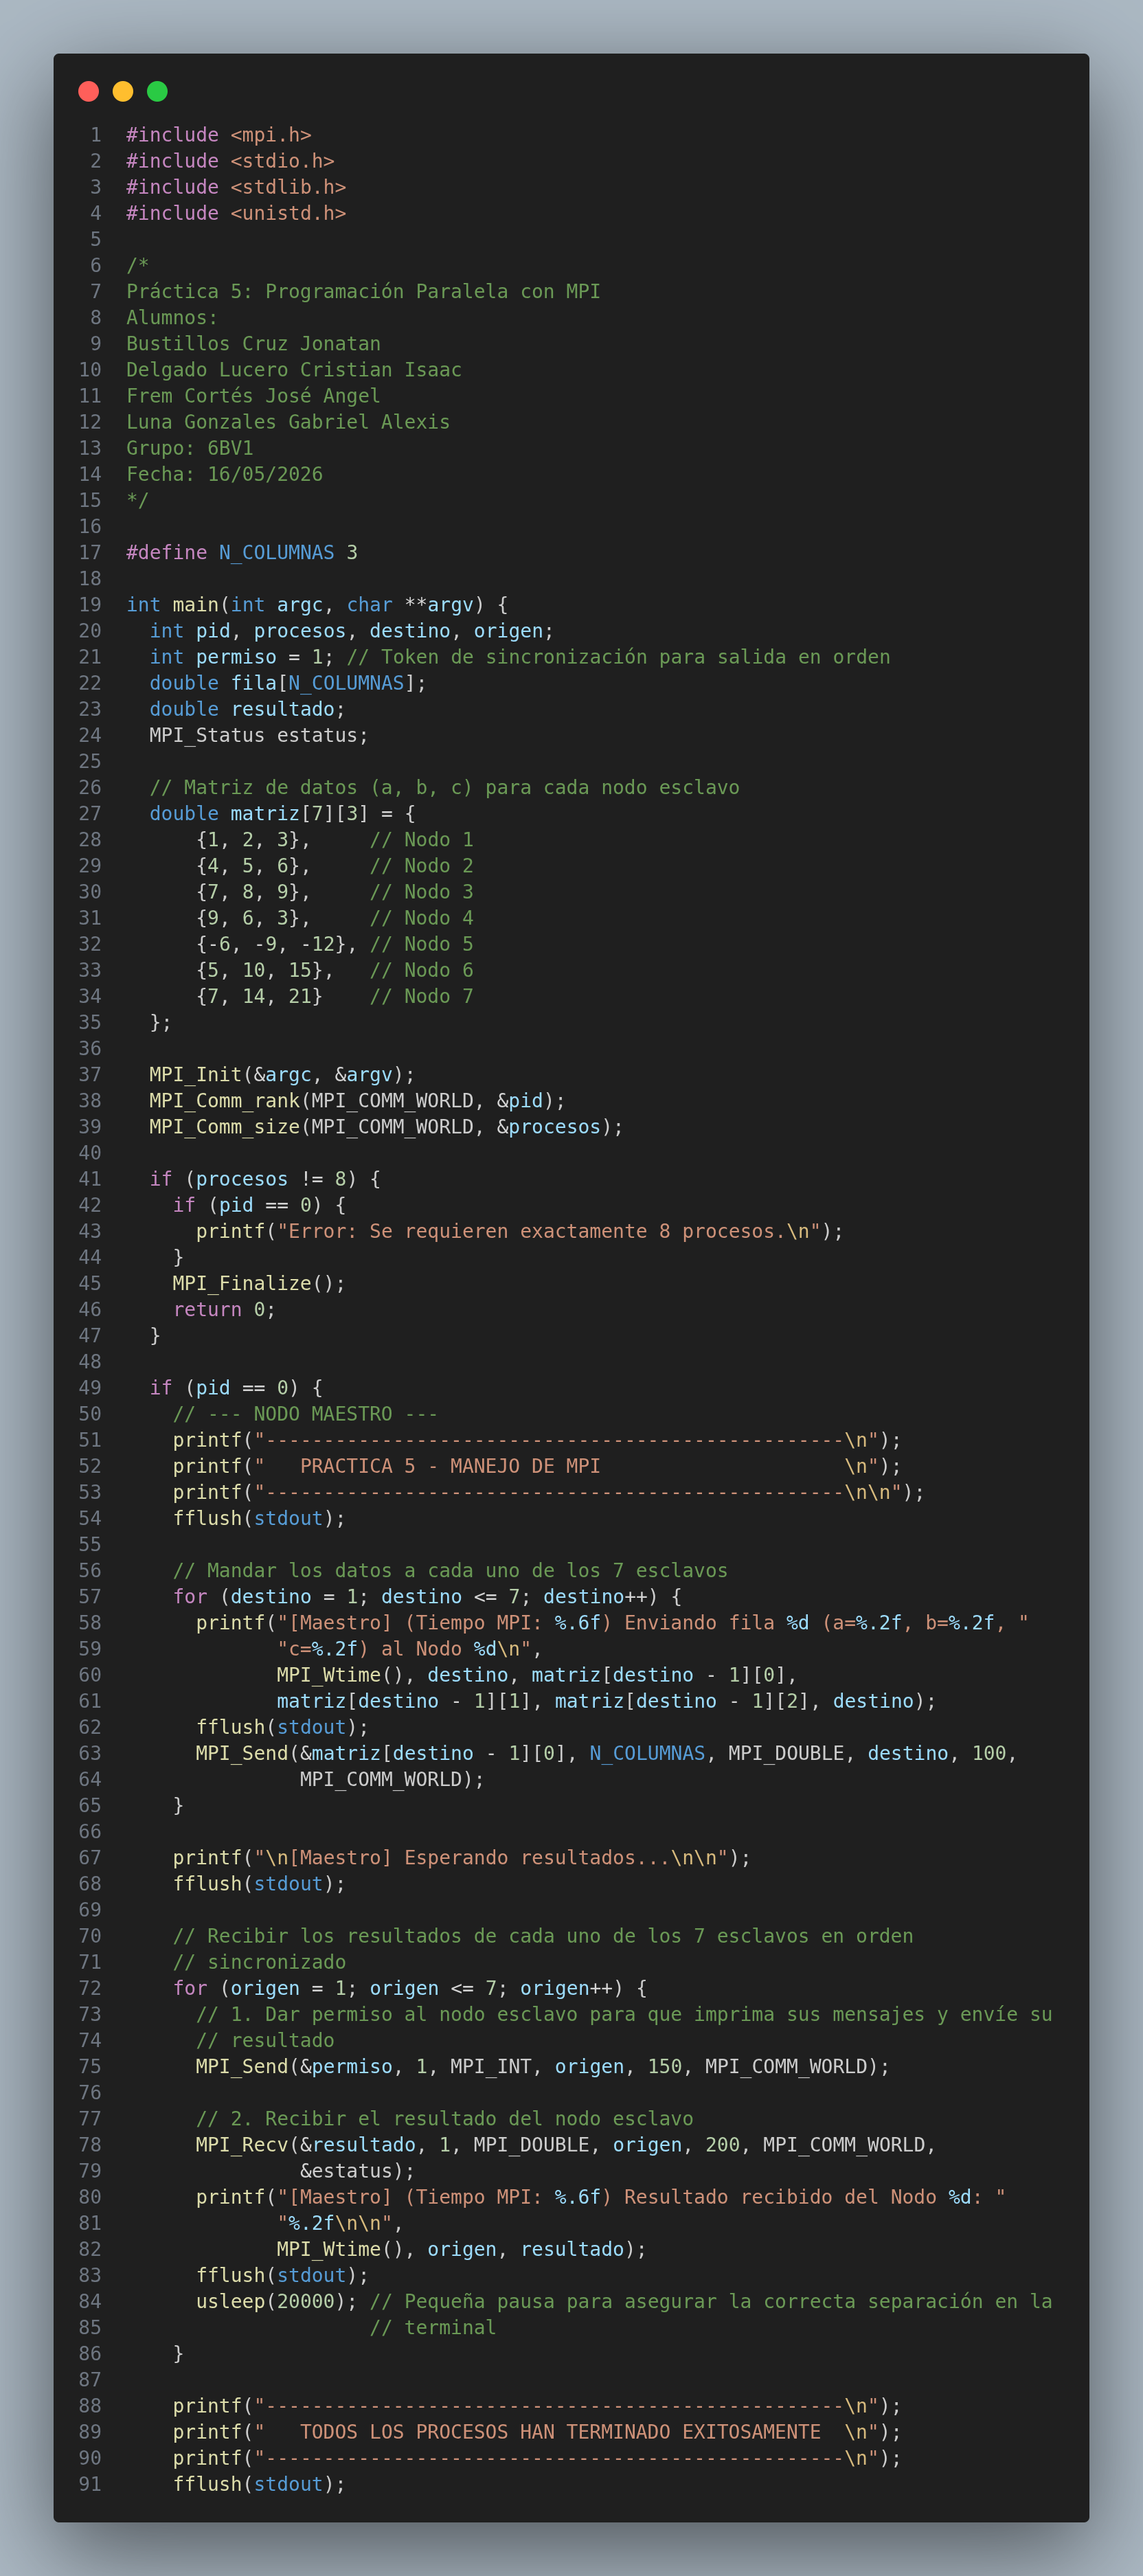
\includegraphics[width=0.75\linewidth]{imagenes/Hako/codigo_main_1.png}
    }
    \caption{Código principal del sistema \texttt{main.c} --- Segmento 1 (superior): inicialización, validación de procesos y configuración del comunicador global. Fuente: Elaboración propia.}
    \label{fig:codigo_main_1_sup}
\end{figure}

Una vez superada la verificación, el flujo se bifurca según el valor de \texttt{pid}. Cuando este identificador es 0, el proceso asume el rol de maestro y ejecuta el bloque que distribuye la carga de trabajo. En primer lugar, el maestro imprime un encabezado informativo y entra en un ciclo \texttt{for} que recorre los destinos del 1 al 7; en cada iteración envía mediante \texttt{MPI\_Send} una fila completa de la matriz usando la etiqueta 100, de modo que cada trabajador recibe sus tres valores flotantes sin ambigüedad. Posteriormente, el maestro inicia una segunda fase de sincronización: por cada trabajador, emite un \textit{token} de permiso con etiqueta 150 para desbloquear la impresión ordenada, y acto seguido recibe el resultado numérico mediante \texttt{MPI\_Recv} con etiqueta 200, mostrando en pantalla el valor devuelto junto con la marca de tiempo de MPI. La Figura~\ref{fig:codigo_main_1_inf} presenta precisamente este segmento inferior del archivo, donde se aprecia la dupla de bucles que gobiernan el envío de datos y la recolección secuencial de resultados.

% --- CÓDIGO MAIN 1: PARTE INFERIOR (lógica del maestro) ---
\begin{figure}[H]
    \centering
    \ContinuedFloat
    \adjustbox{trim=0 0 0 {0.53\height}, clip}{
        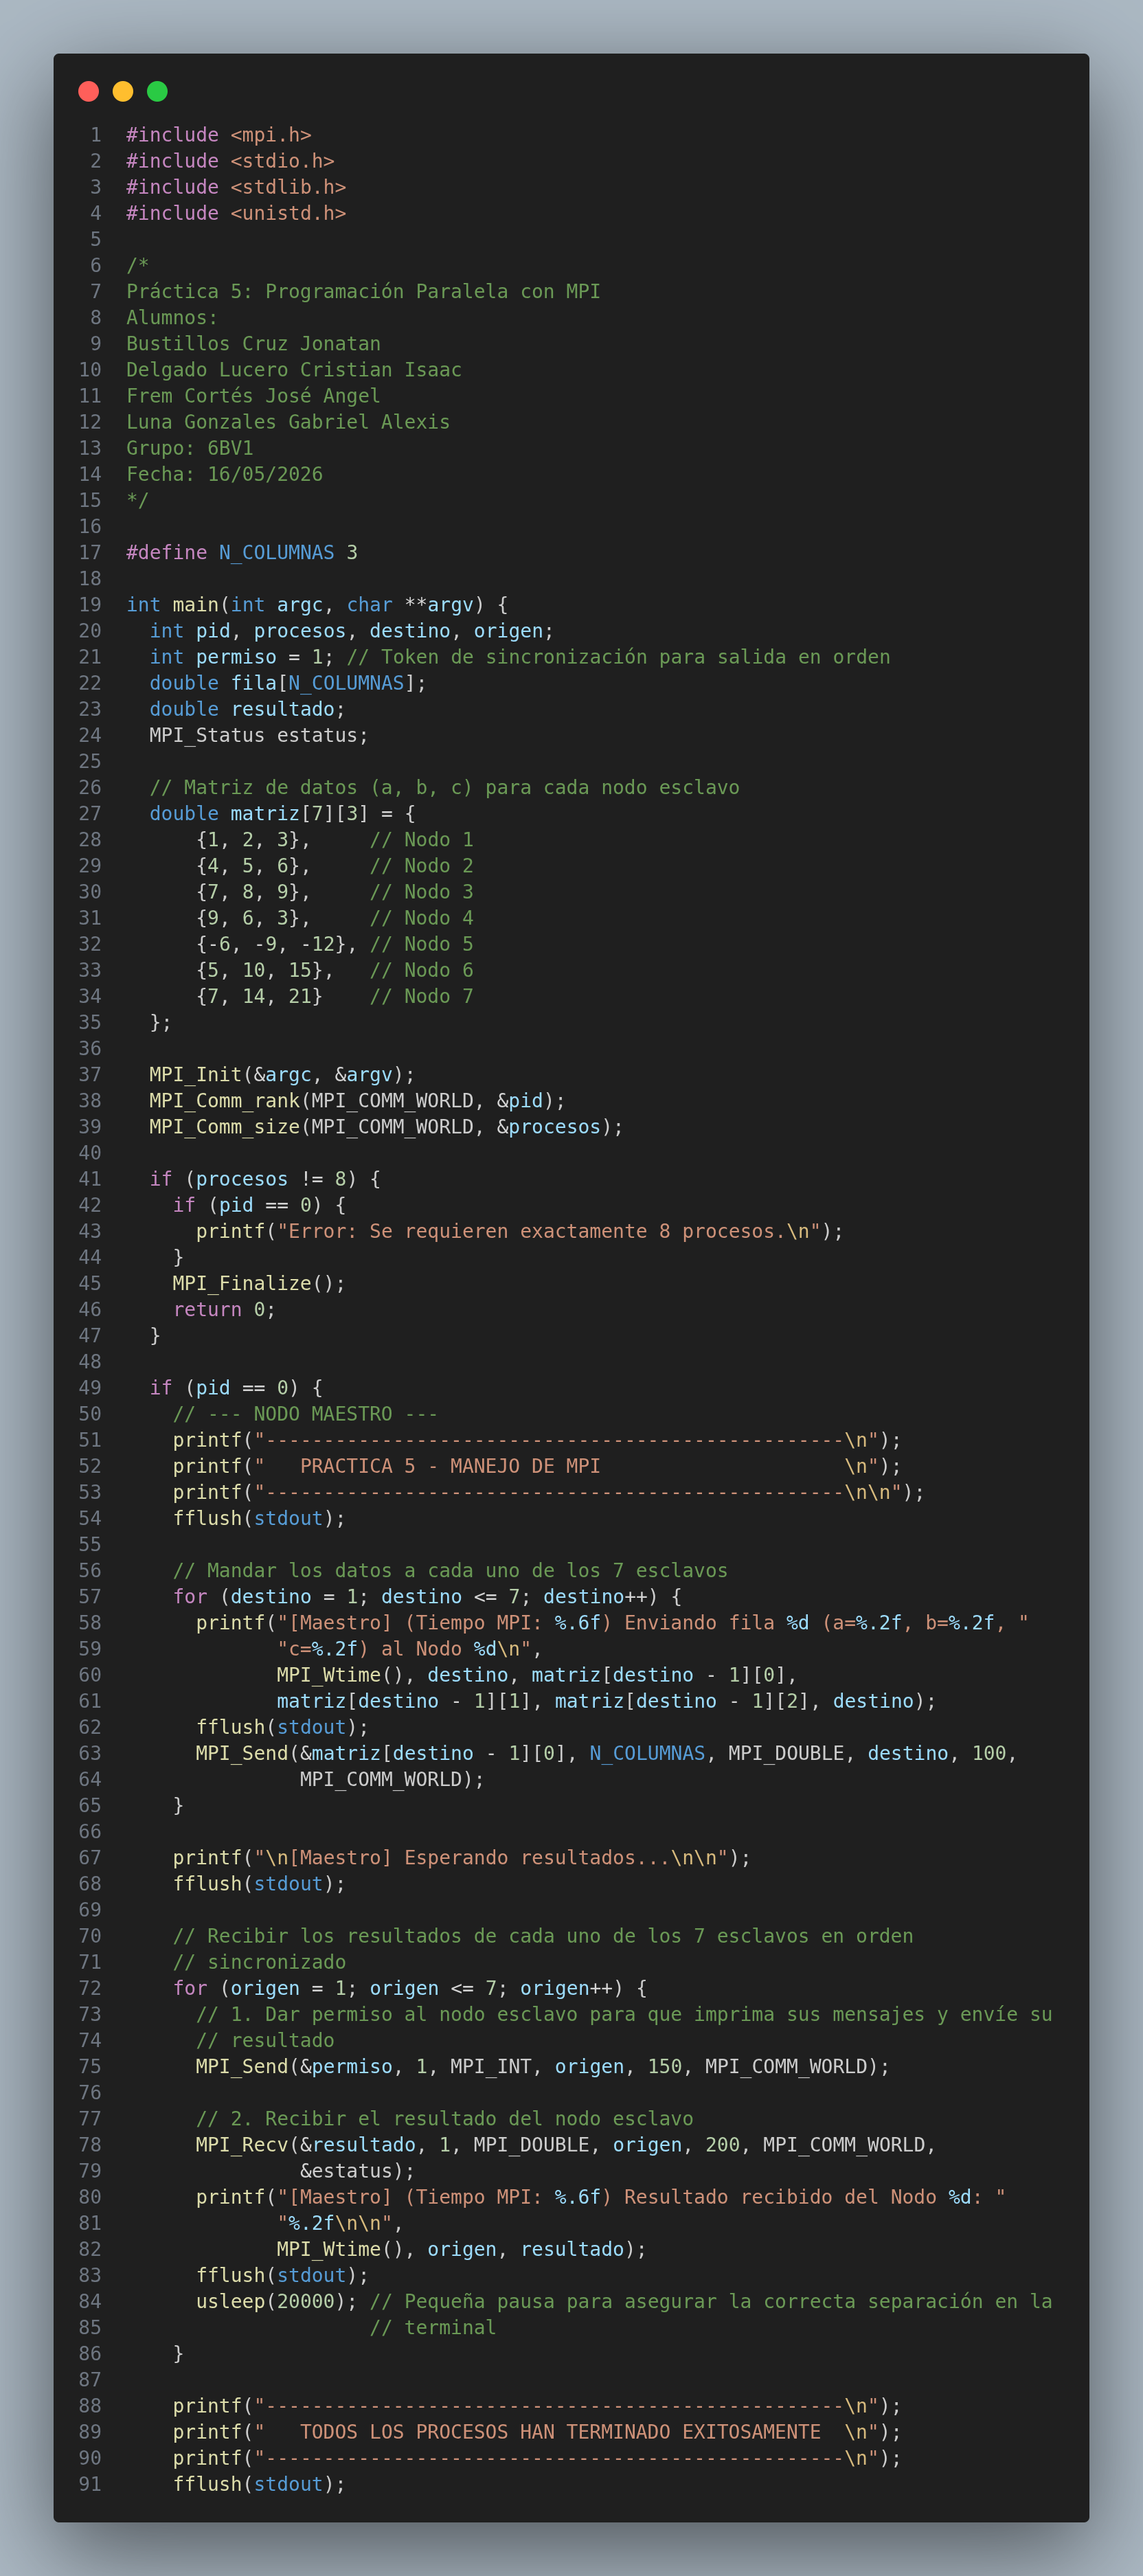
\includegraphics[width=0.85\linewidth]{imagenes/Hako/codigo_main_1.png}
    }
    \caption{Código principal del sistema \texttt{main.c} --- Segmento 1 (inferior): lógica del nodo maestro, distribución de datos y recepción de resultados. Fuente: Elaboración propia.}
    \label{fig:codigo_main_1_inf}
\end{figure}

Del lado de los procesos trabajadores, cada uno ejecuta un bloque condicional exclusivo determinado por su \texttt{pid}. Los nodos 1 y 2 ilustran el patrón común que se repite a lo largo de todo el conjunto: primero reciben su fila de datos mediante \texttt{MPI\_Recv} con etiqueta 100, aplican la operación aritmética que les corresponde y permanecen a la espera del \textit{token} de permiso para escribir en la salida estándar. El nodo 1 calcula la suma $a+b+c$, mientras que el nodo 2 resuelve la expresión $a-b+c$; en ambos casos, tras imprimir los valores recibidos y el resultado obtenido, devuelven la cantidad computada al maestro a través de \texttt{MPI\_Send} con etiqueta 200. Este esquema de recepción-cálculo-espera-envío asegura que cada trabajador opere de forma autónoma y que sus mensajes no se entremezclen en la terminal gracias al control jerárquico del maestro. La Figura~\ref{fig:codigo_main_2_sup} muestra estas dos primeras ramas del bloque condicional, correspondientes a los trabajadores 1 y 2.

% --- CÓDIGO MAIN 2: PARTE SUPERIOR (nodos 1 y 2) ---
\begin{figure}[H]
    \centering
    \adjustbox{trim=0 {0.50\height} 0 0, clip}{
        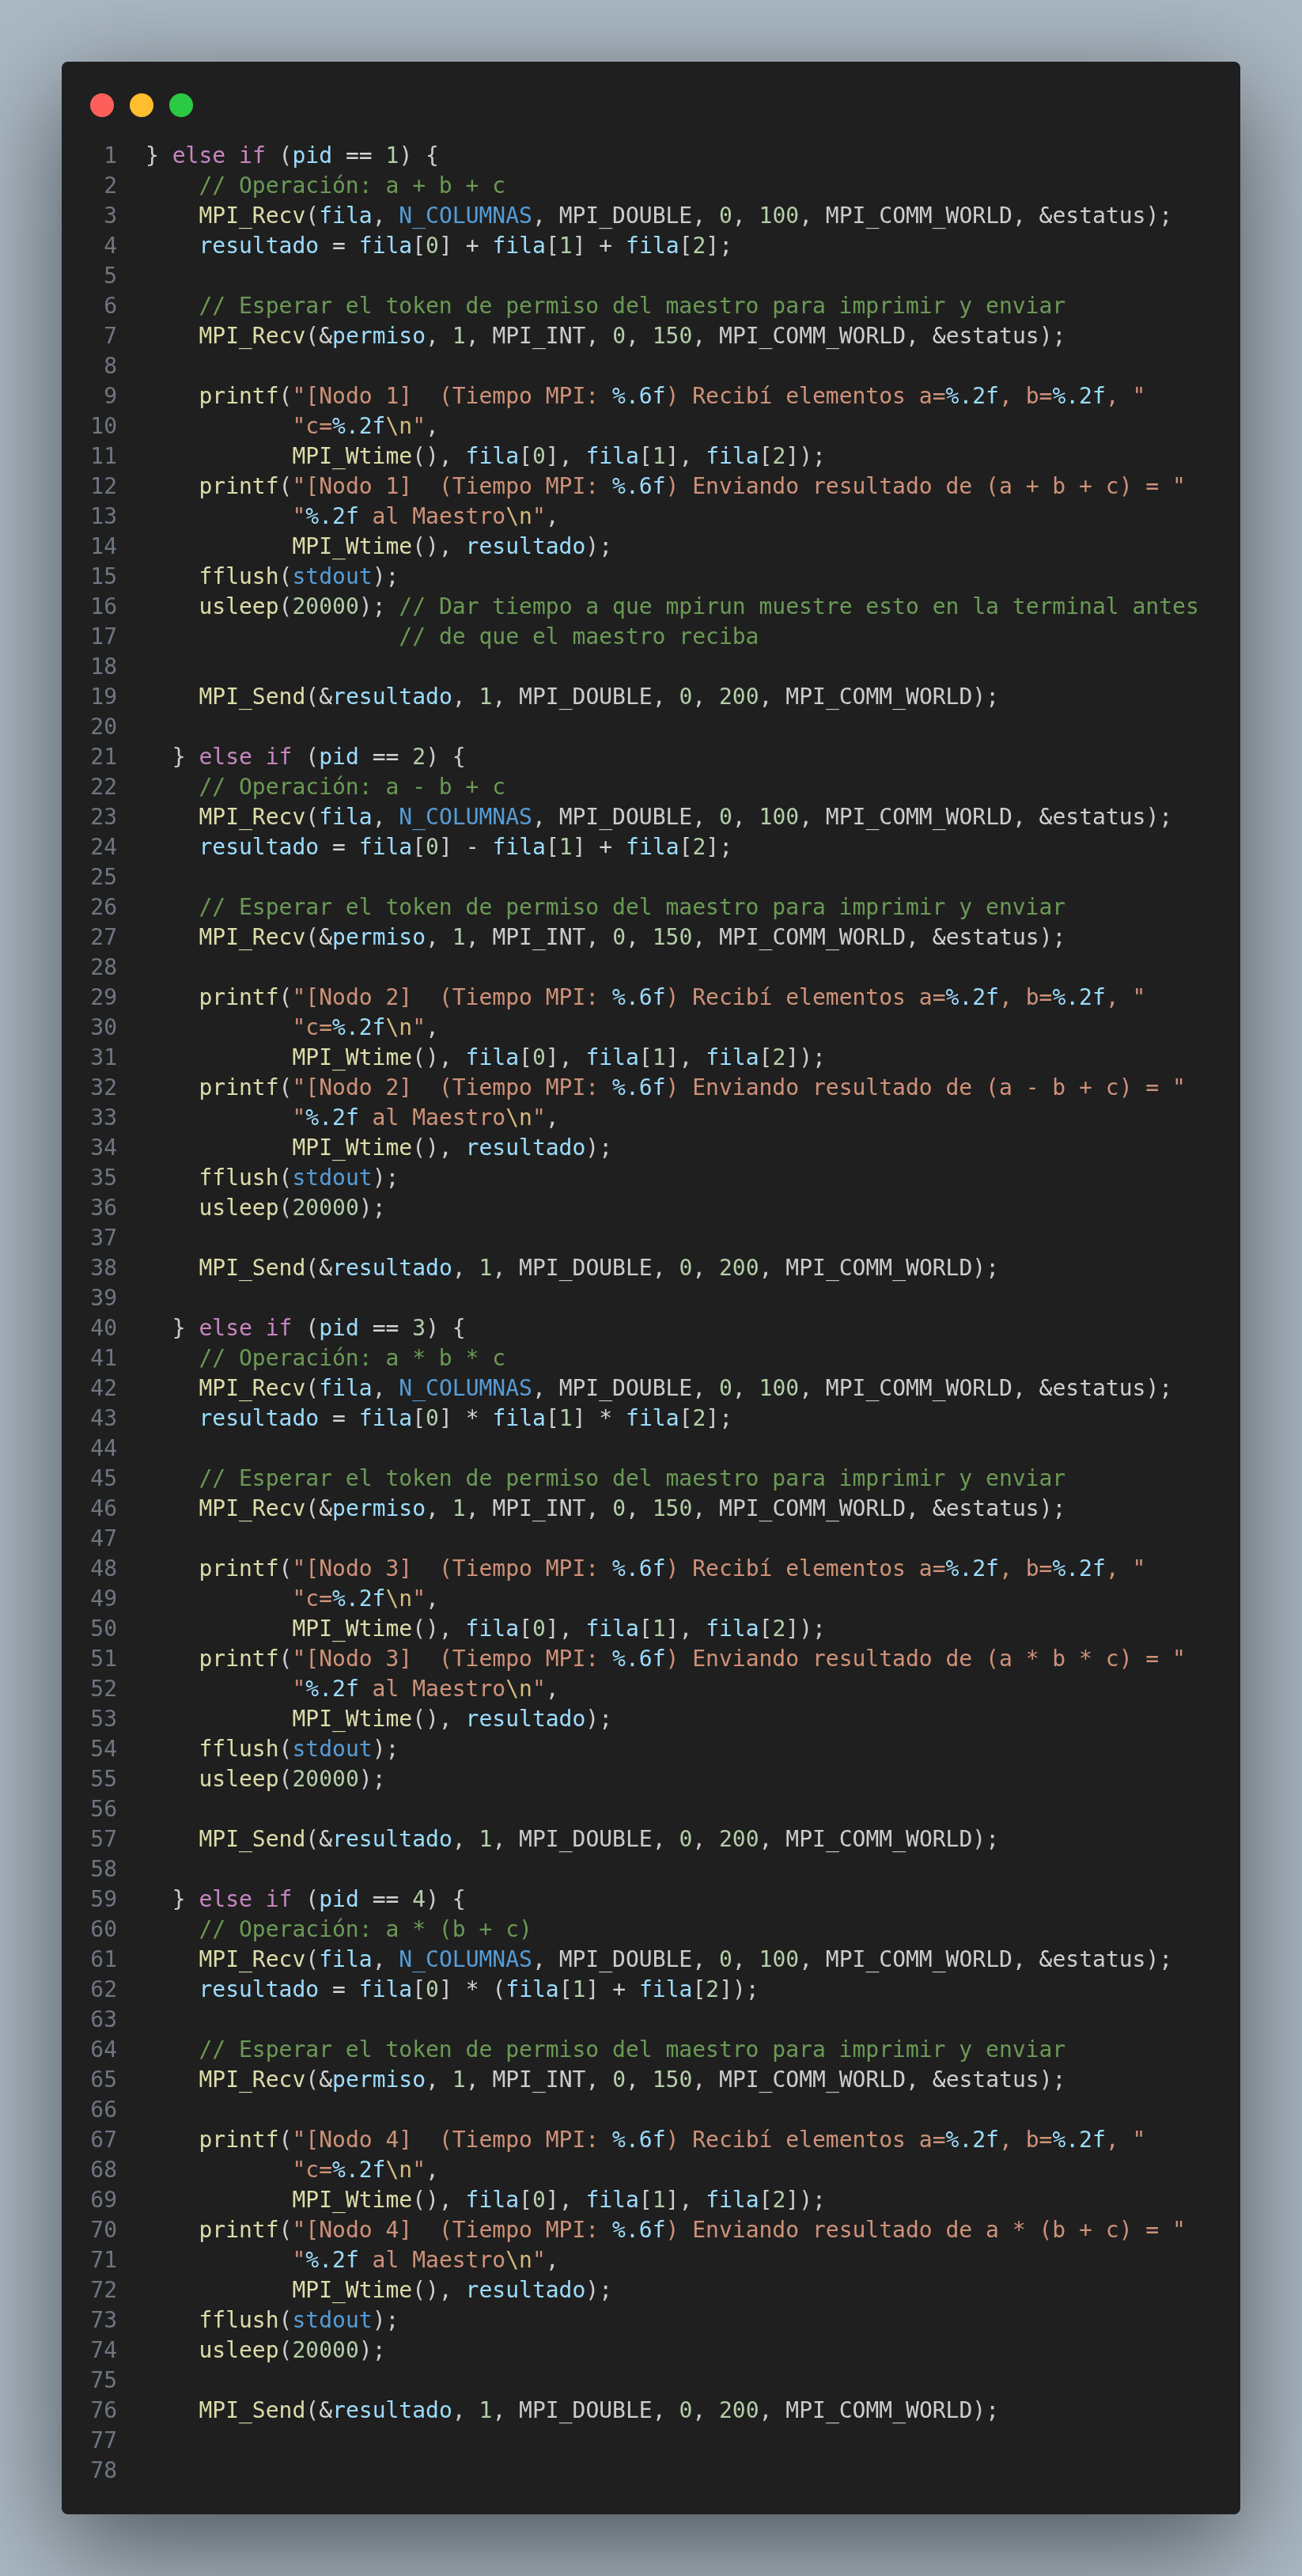
\includegraphics[width=0.85\linewidth]{imagenes/Hako/codigo_main_2.png}
    }
    \caption{Código principal del sistema \texttt{main.c} --- Segmento 2 (superior): procesamiento de los nodos trabajadores 1 y 2. Fuente: Elaboración propia.}
    \label{fig:codigo_main_2_sup}
\end{figure}

De manera análoga, los nodos 3 y 4 extienden la lógica anterior hacia operaciones de mayor complejidad algebraica. El trabajador 3 realiza el producto $a \cdot b \cdot c$, mientras que el trabajador 4 evalúa la expresión $a \cdot (b+c)$, lo cual exige el uso de paréntesis para respetar la precedencia de operadores en el código fuente. En ambos fragmentos se conserva la misma secuencia de llamadas MPI: recepción de la fila, espera del \textit{token} con etiqueta 150, impresión sincronizada de los mensajes y remisión del resultado al proceso 0 mediante la etiqueta 200. Esta uniformidad en la interfaz de comunicación simplifica considerablemente el diseño del maestro, ya que puede anticipar el tamaño y el tipo de cada mensaje sin necesidad de negociación dinámica. La Figura~\ref{fig:codigo_main_2_inf} captura exactamente estas dos ramas, permitiendo contrastar las diferencias en las fórmulas sin perder de vista la identidad estructural del protocolo.

% --- CÓDIGO MAIN 2: PARTE INFERIOR (nodos 3 y 4) ---
\begin{figure}[H]
    \centering
    \ContinuedFloat
    \adjustbox{trim=0 0 0 {0.50\height}, clip}{
        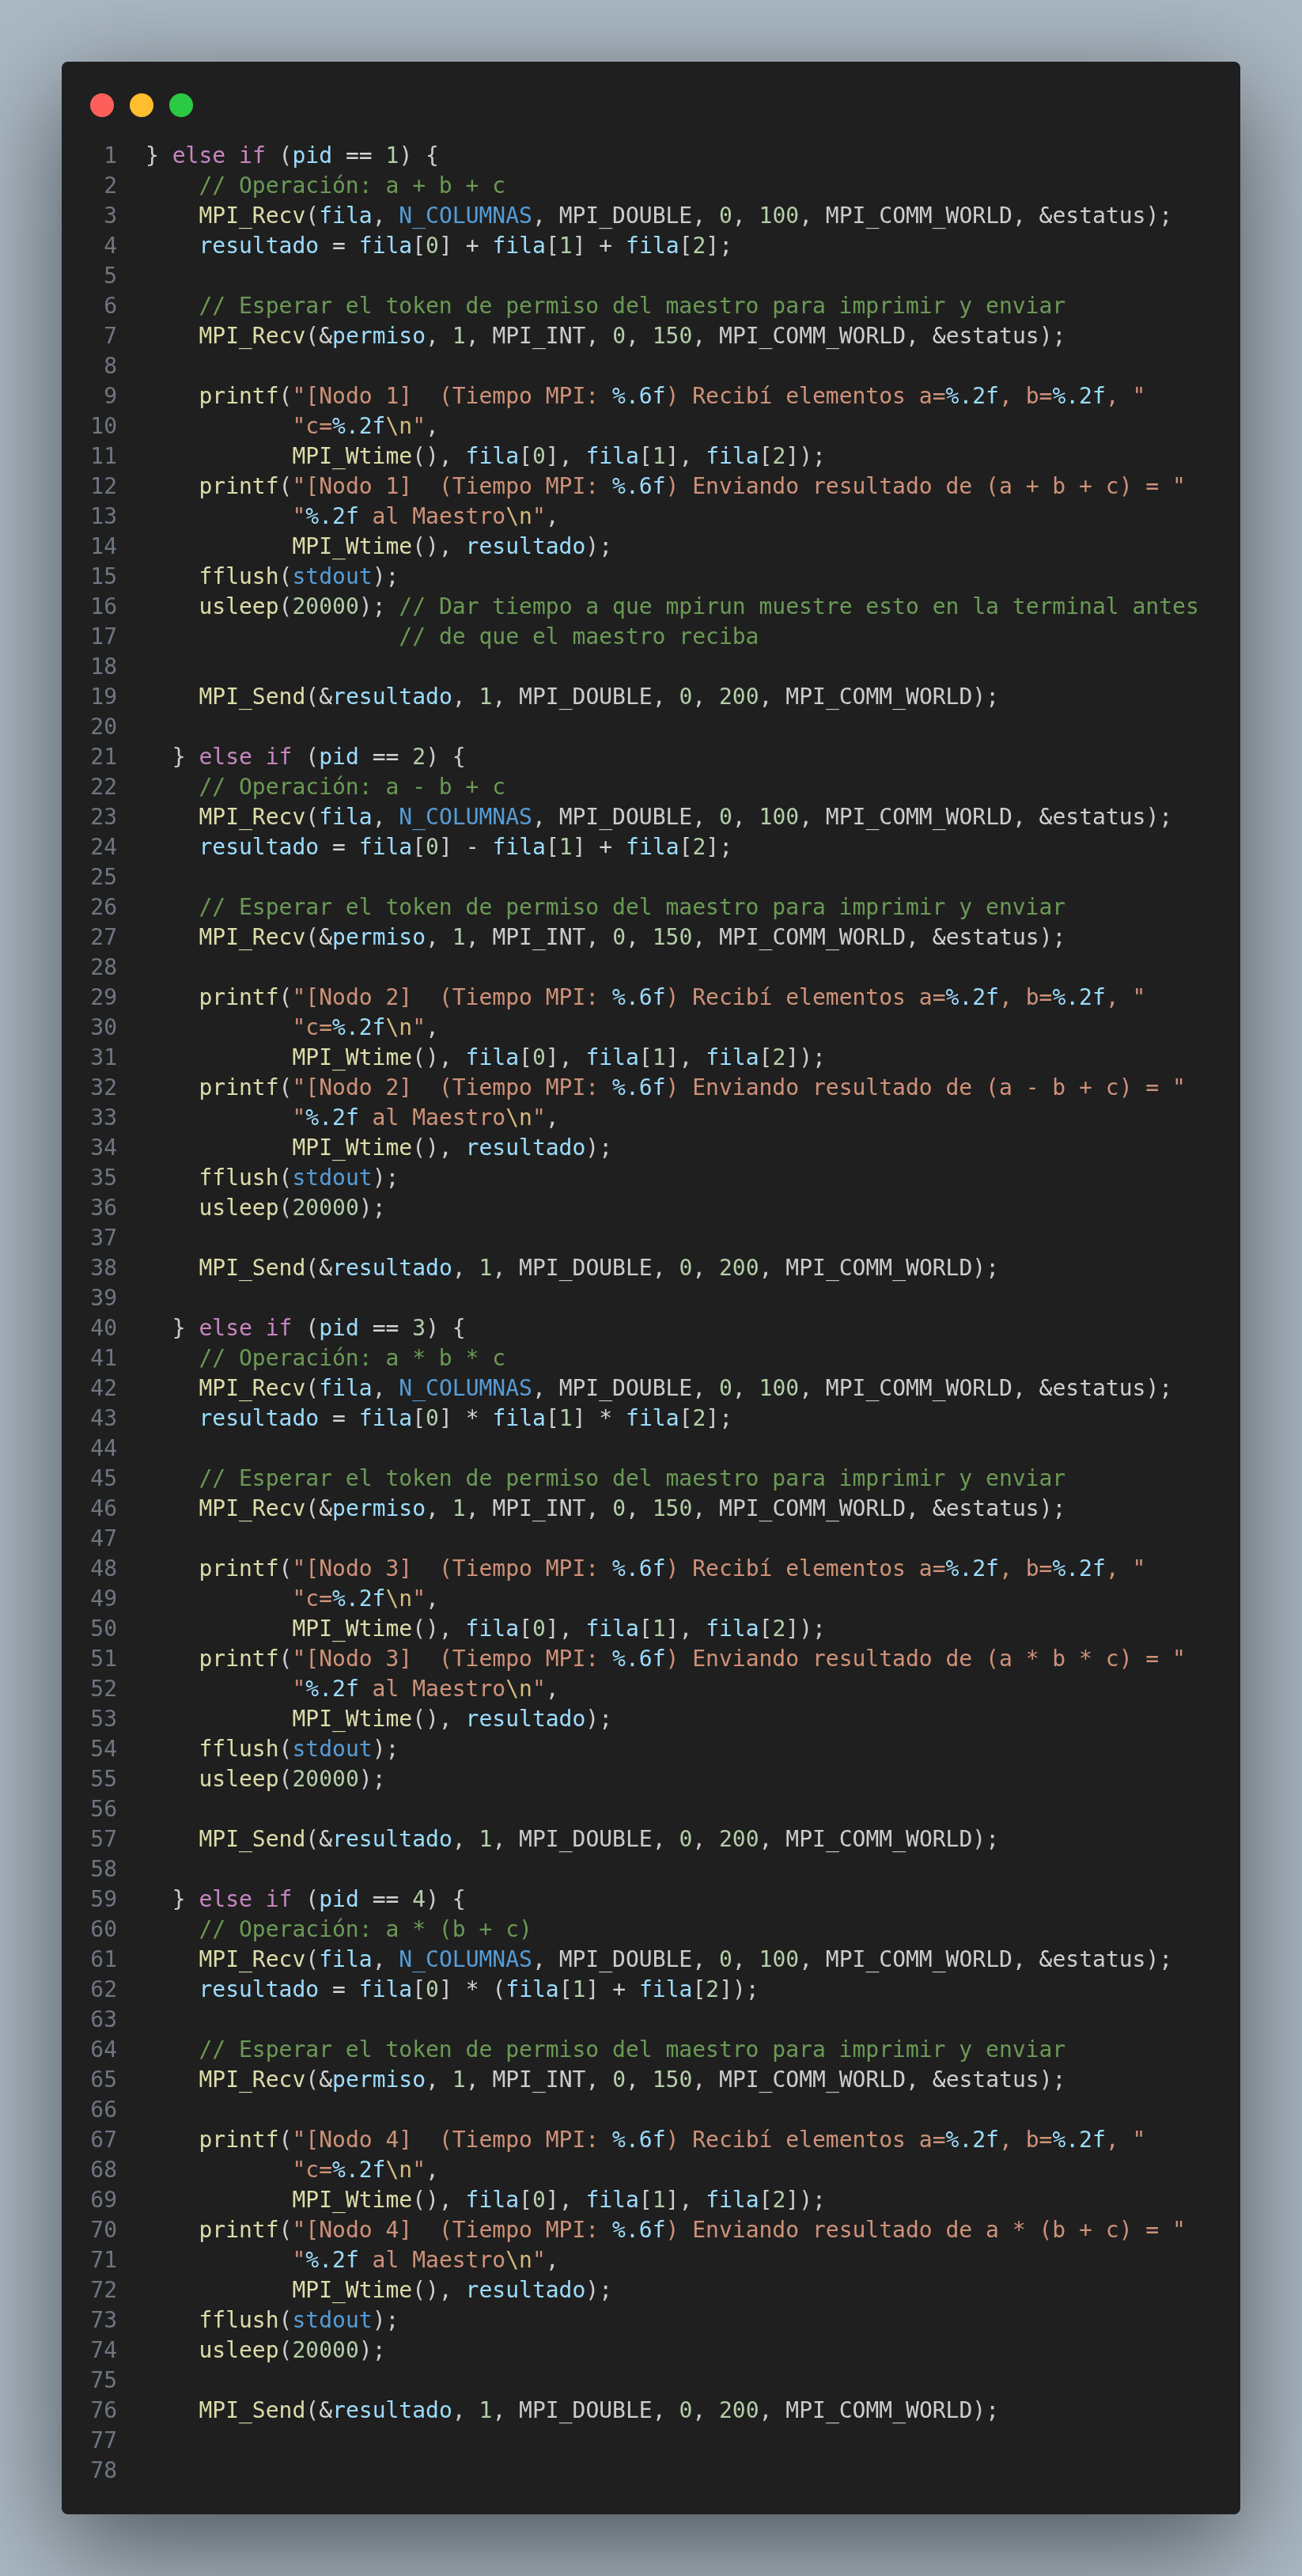
\includegraphics[width=0.85\linewidth]{imagenes/Hako/codigo_main_2.png}
    }
    \caption{Código principal del sistema \texttt{main.c} --- Segmento 2 (inferior): procesamiento de los nodos trabajadores 3 y 4. Fuente: Elaboración propia.}
    \label{fig:codigo_main_2_inf}
\end{figure}

Los trabajadores 5 y 6 continúan con la misma metodología, aunque las expresiones que evalúan introducen combinaciones aritméticas que requieren mayor atención en la traducción a instrucciones C. El nodo 5 computa $a \cdot b - b \cdot c$, descomponiendo la operación en dos productos parciales cuyo resultado se resta; por su parte, el nodo 6 eleva al cuadrado la suma $(a+b)$ y multiplica el resultado por $c$, lo cual se implementa replicando el factor $(a+b)$ en lugar de invocar una función de potencia. Ambos procesos respetan el contrato de comunicación previamente establecido: reciben sus valores, esperan el permiso del maestro, imprimen sus mensajes con la marca \texttt{MPI\_Wtime} y envían la respuesta final. En la Figura~\ref{fig:codigo_main_3_sup} se aprecia este par de bloques, donde la legibilidad del código permite identificar claramente las diferencias entre las fórmulas sin perder la homogeneidad del patrón de mensajes.

% --- CÓDIGO MAIN 3: PARTE SUPERIOR (nodos 5 y 6) ---
\begin{figure}[H]
    \centering
    \adjustbox{trim=0 {0.40\height} 0 0, clip}{
        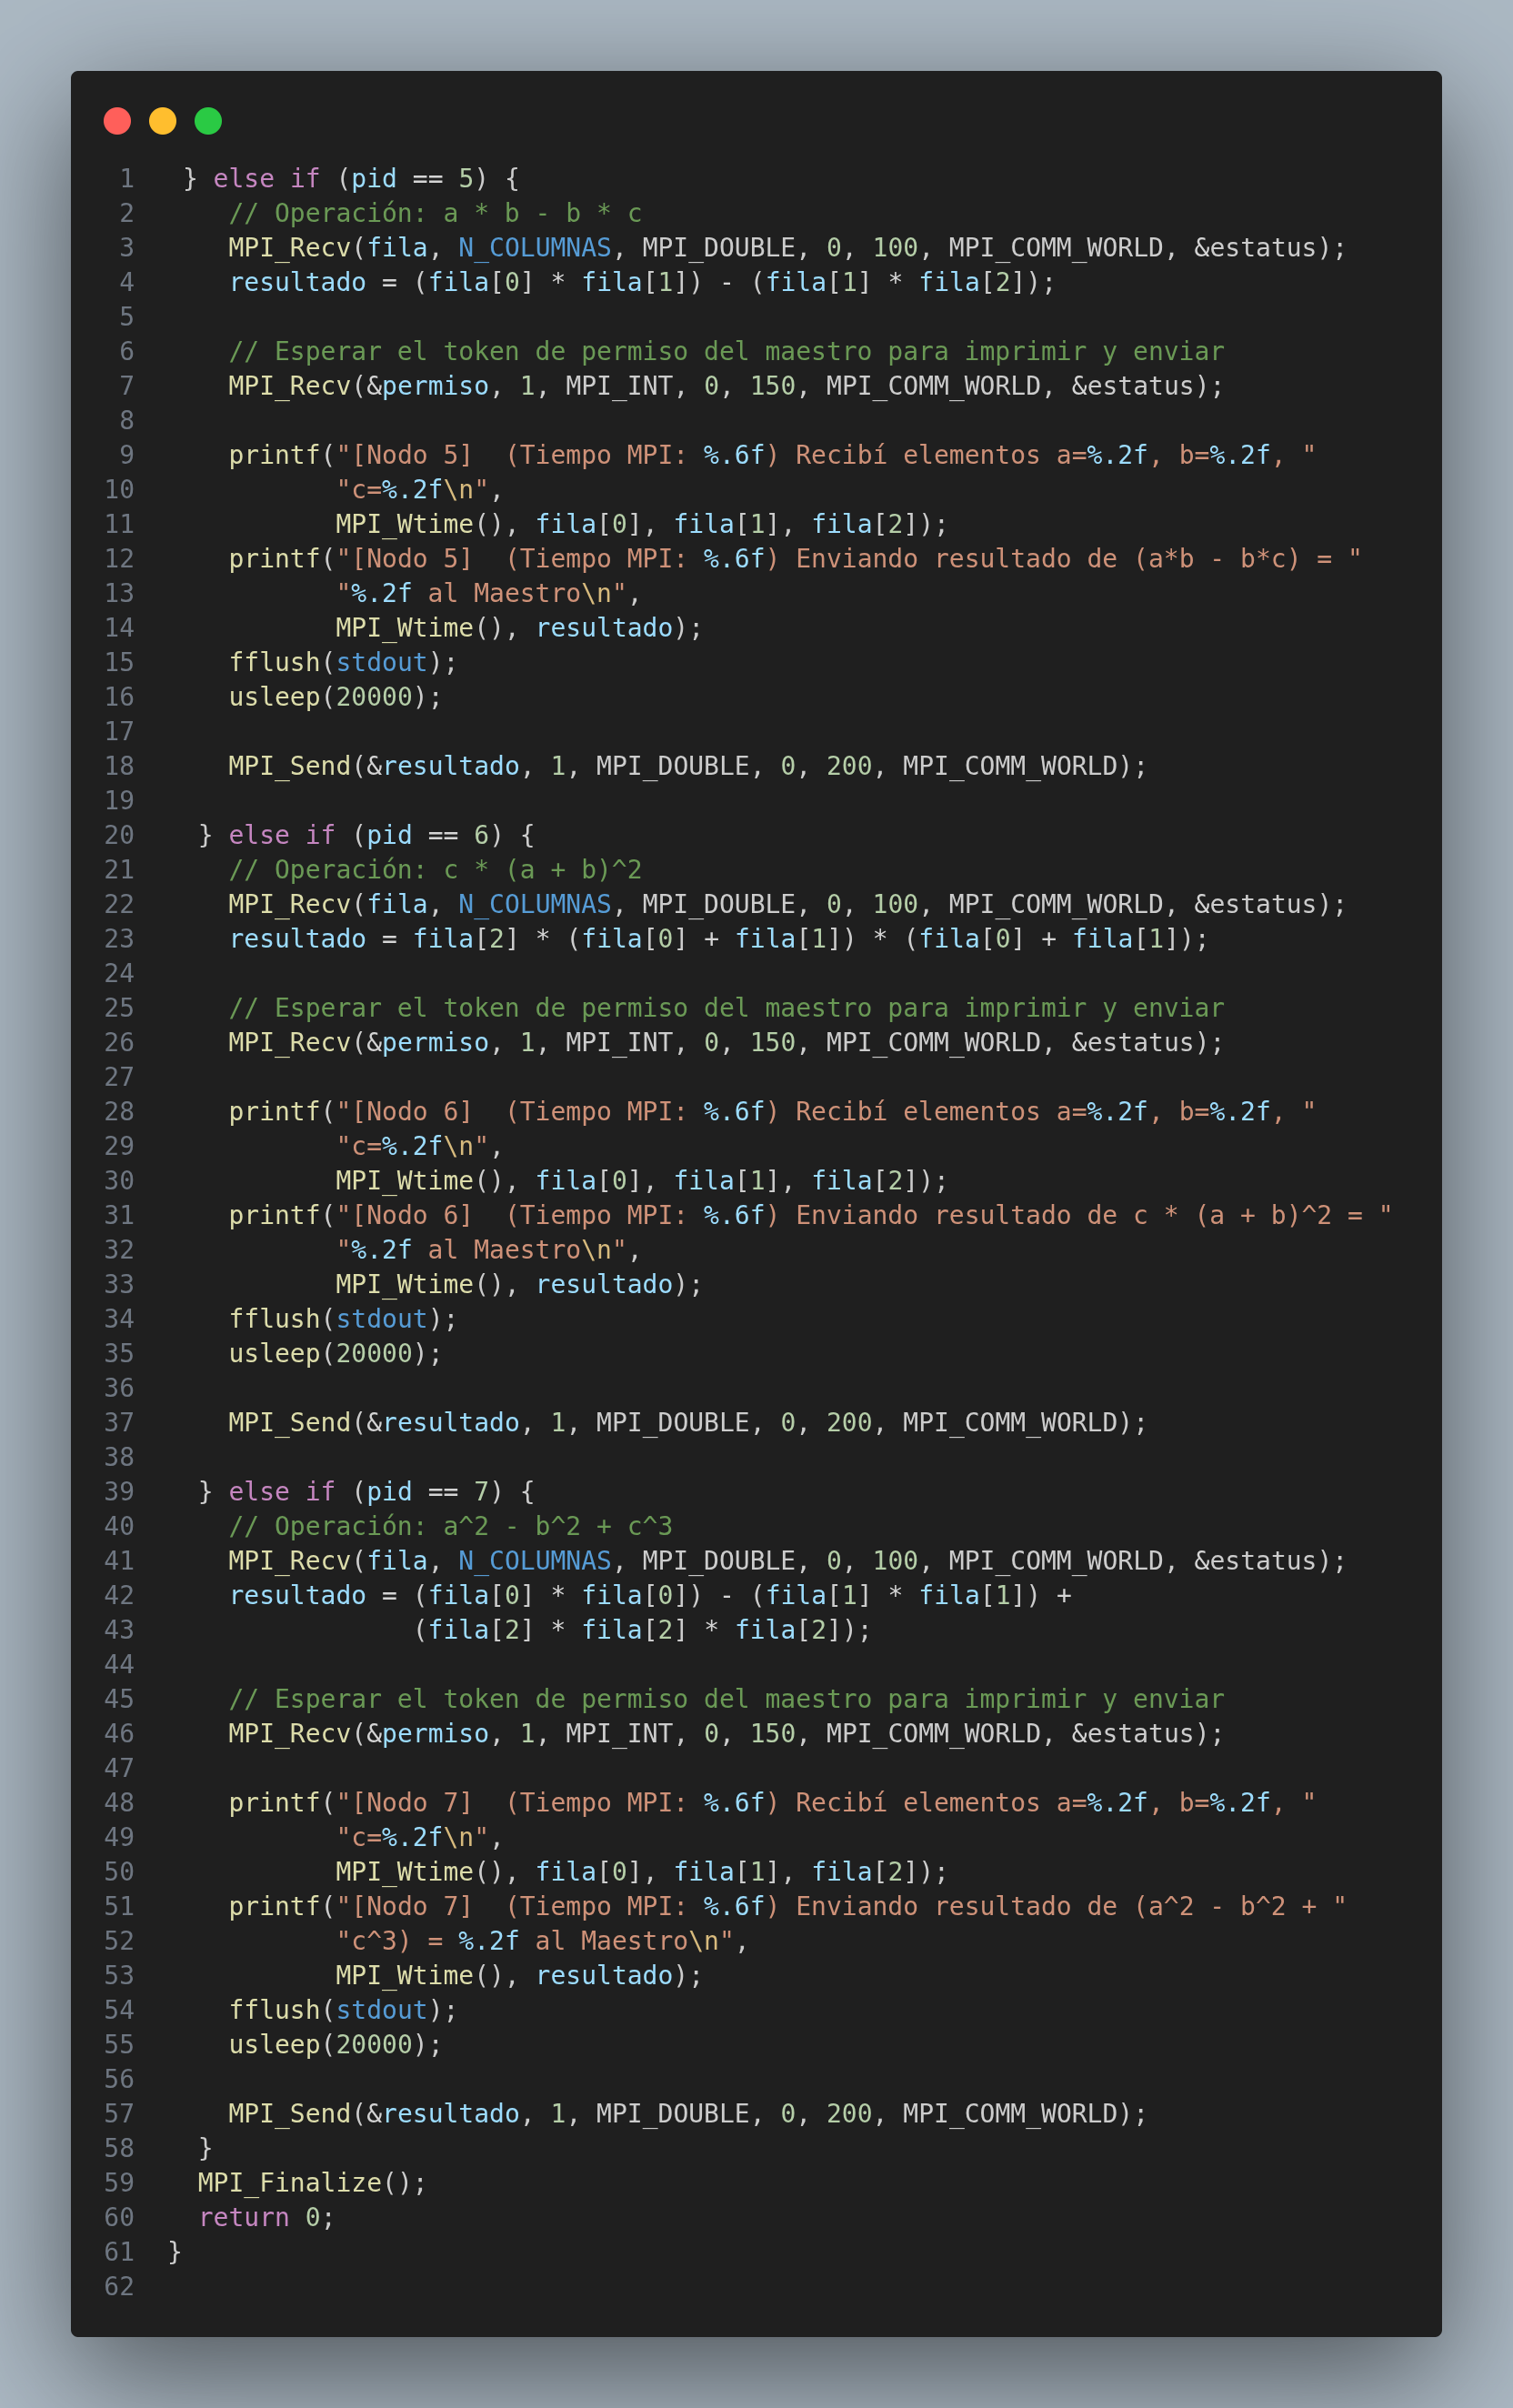
\includegraphics[width=0.85\linewidth]{imagenes/Hako/codigo_main_3.png}
    }
    \caption{Código principal del sistema \texttt{main.c} --- Segmento 3 (superior): procesamiento de los nodos trabajadores 5 y 6. Fuente: Elaboración propia.}
    \label{fig:codigo_main_3_sup}
\end{figure}

Finalmente, el nodo 7 cierra el conjunto de trabajadores evaluando la expresión $a^2 - b^2 + c^3$, que se traduce en el código como una serie de multiplicaciones encadenadas para evitar dependencias de bibliotecas matemáticas adicionales. Tras completar su cálculo y enviar el resultado al maestro, el programa alcanza la zona de clausura común a todos los procesos, donde se invoca \texttt{MPI\_Finalize} para liberar los recursos del entorno de paso de mensajes y se retorna el valor 0, indicando una terminación exitosa. Este último paso es indispensable, ya que omitir la finalización correcta de MPI podría dejar procesos zombis o buffers de comunicación sin liberar en el sistema operativo subyacente. La Figura~\ref{fig:codigo_main_3_inf} exhibe la rama del trabajador 7 junto con las instrucciones de cierre, completando así la visión integral del archivo \texttt{main.c}.

% --- CÓDIGO MAIN 3: PARTE INFERIOR (nodo 7 y clausura) ---
\begin{figure}[H]
    \centering
    \ContinuedFloat
    \adjustbox{trim=0 0 0 {0.60\height}, clip}{
        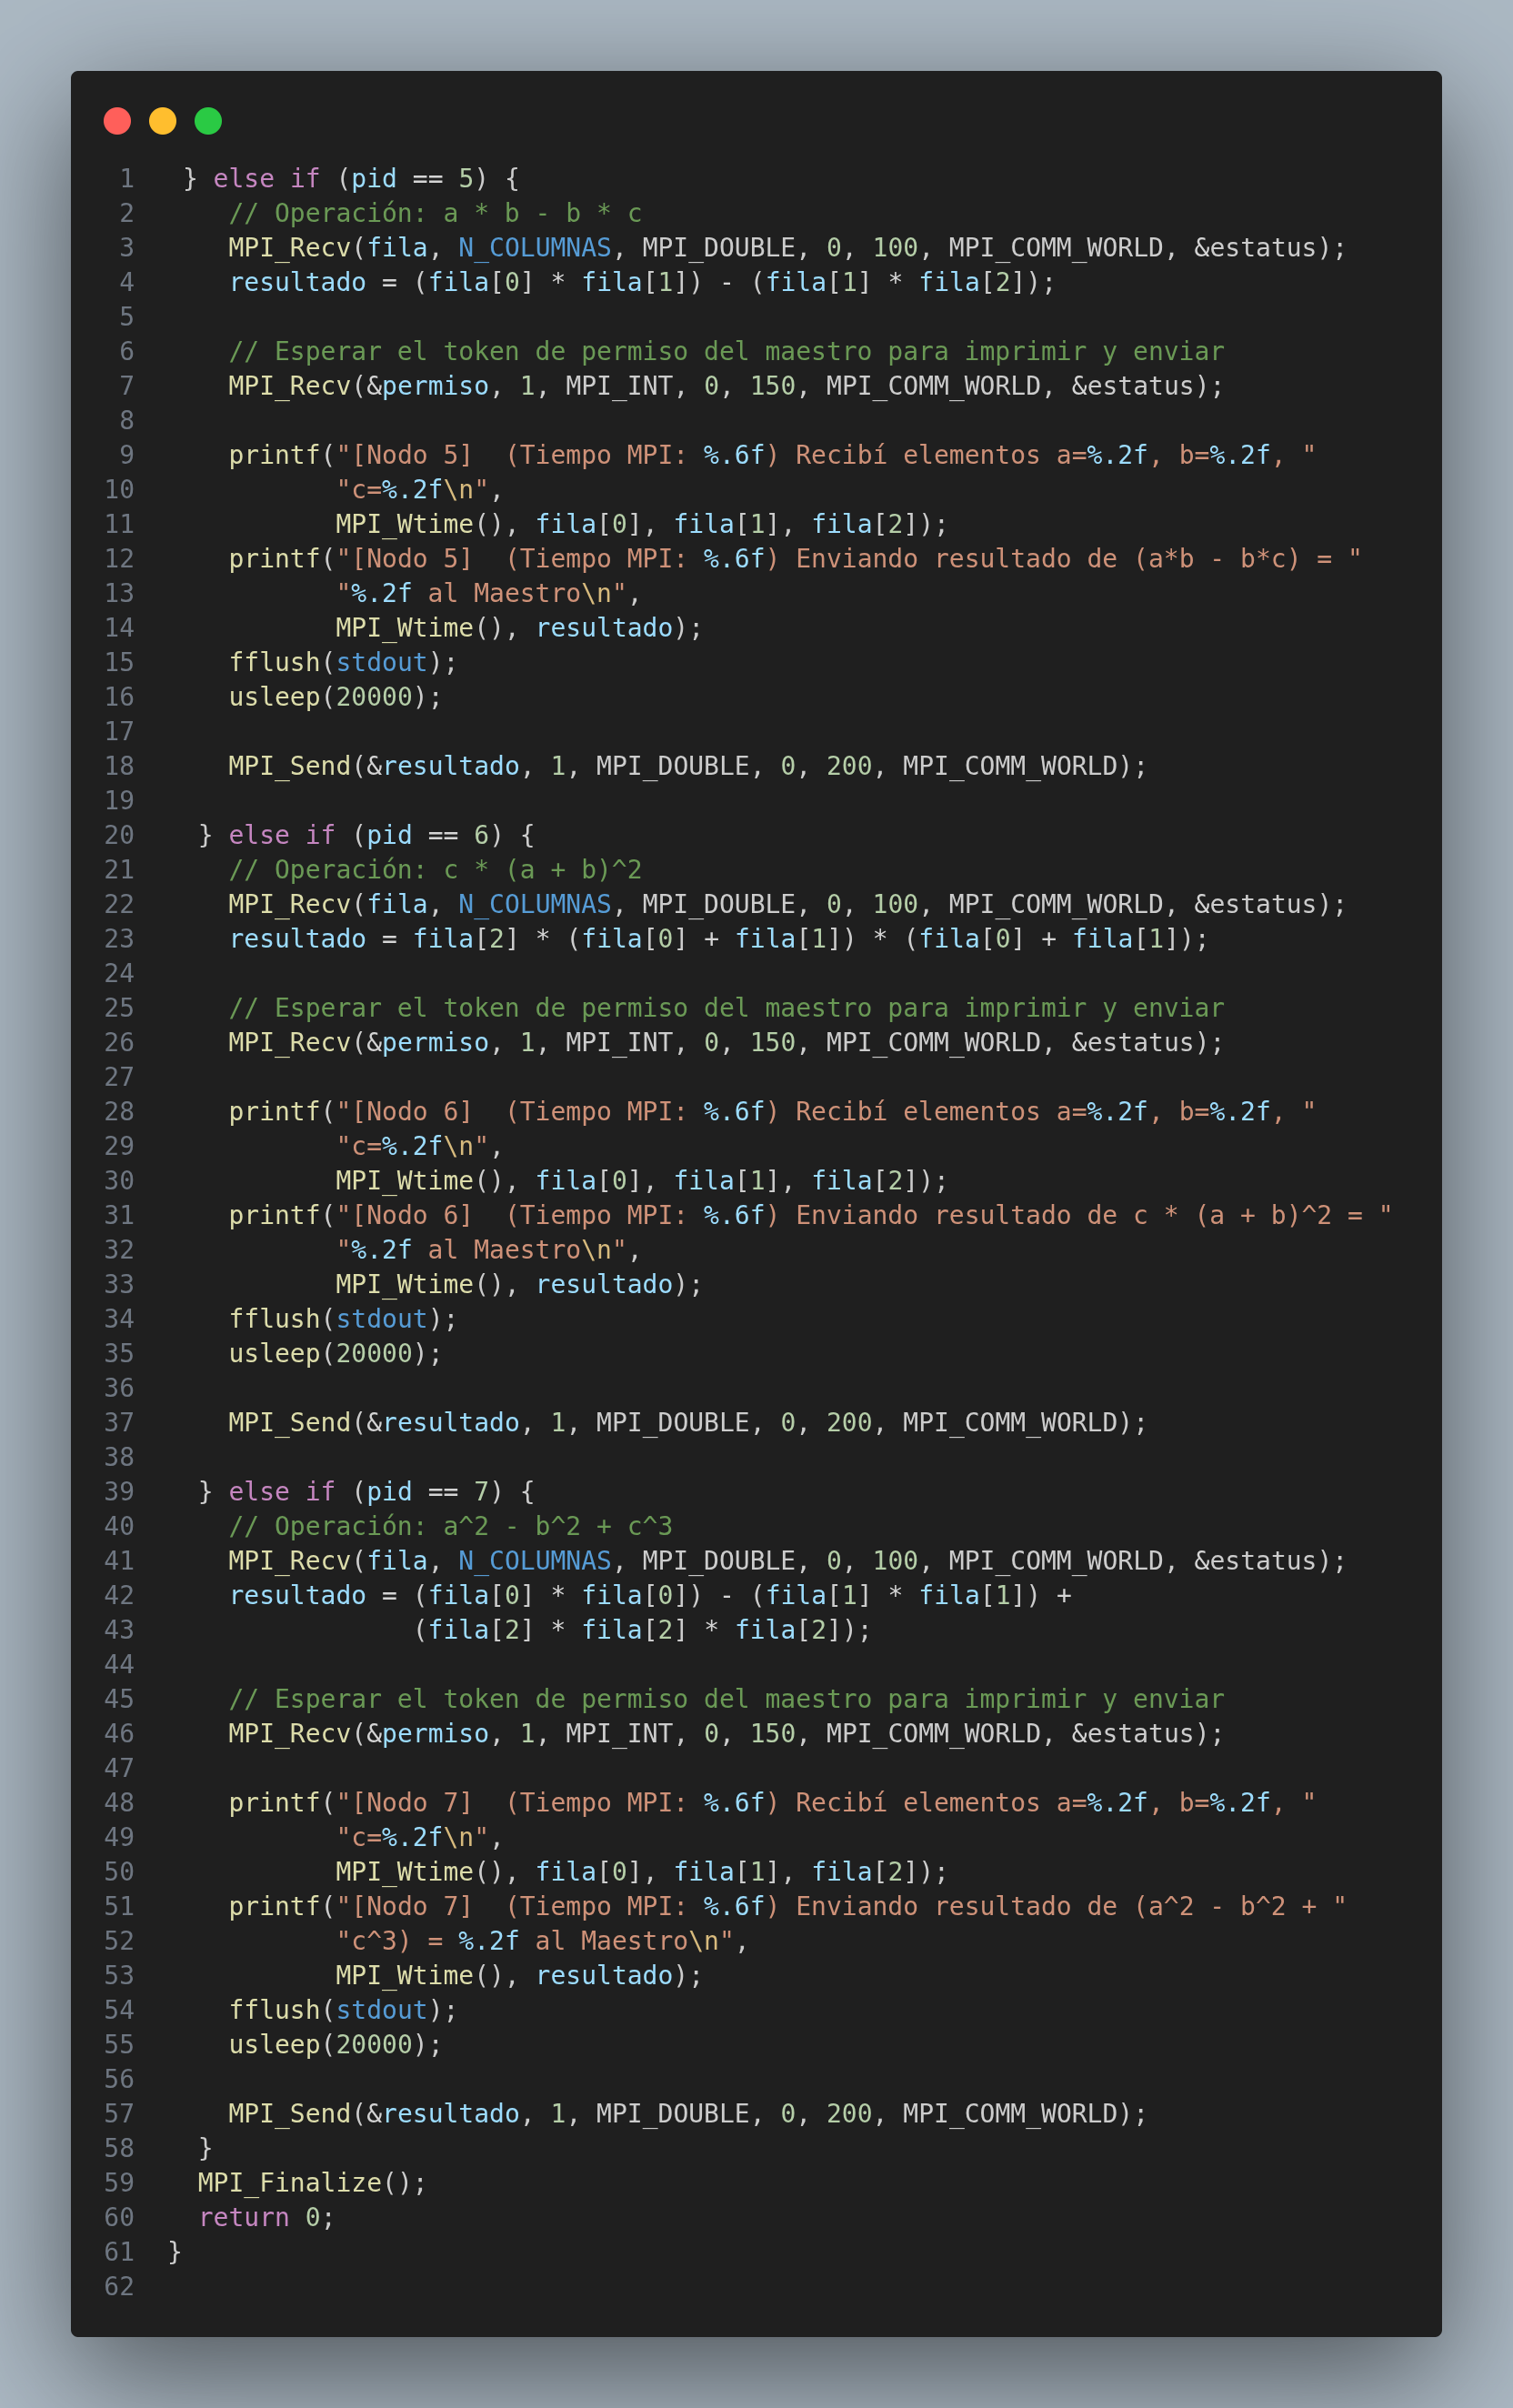
\includegraphics[width=0.85\linewidth]{imagenes/Hako/codigo_main_3.png}
    }
    \caption{Código principal del sistema \texttt{main.c} --- Segmento 3 (inferior): procesamiento del nodo trabajador 7 y clausura del entorno MPI. Fuente: Elaboración propia.}
    \label{fig:codigo_main_3_inf}
\end{figure}

\section{Evidencia de Ejecución}

% ==========================================
% SUGERENCIAS
% ==========================================
% 1. Se recomienda incluir CAPTURAS DE PANTALLA DE LA EJECUCIÓN.
%    - Podrías mostrar el comando que usaste para compilar.
%    - Sería útil mostrar el comando que usaste para ejecutar (mpirun/mpiexec).
%    - Se sugiere mostrar la SALIDA del programa con diferentes números de procesos.
%
% 2. Opcionalmente, COMPARACIÓN DE RESULTADOS.
%    - ¿Los resultados con 2, 4 y 8 procesos son consistentes?
%    - ¿Se observa mejora en el tiempo de ejecución?
%
% 3. Se sugiere una TABLA DE RESULTADOS.
%    - Podrías usar el entorno `table` para presentar tiempos de ejecución.
%    Ejemplo:
%    \begin{table}[h]
%    \centering
%    \begin{tabular}{|c|c|c|}
%    \hline
%    \textbf{Procesos} & \textbf{Tamaño} & \textbf{Tiempo (s)} \\
%    \hline
%    1 & 1000 & 0.05 \\
%    2 & 1000 & 0.03 \\
%    4 & 1000 & 0.02 \\
%    \hline
%    \end{tabular}
%    \caption{Tiempos de ejecución para N=1000}
%    \end{table}
%
% 4. GRÁFICAS (completamente opcional, pero muy profesional).
%    - Si lo deseas, podrías incluir gráficas de speedup o eficiencia.
%    - Se recomienda guardar las imágenes en la carpeta imagenes/.
% ==========================================

% TIP: Para insertar imágenes, podrías usar:
%      \begin{figure}[h]
%      \centering
%      \includegraphics[width=0.8\textwidth]{imagenes/captura1.png}
%      \caption{Ejecución con 4 procesos}
%      \end{figure}
%
%      Se sugiere verificar que la imagen exista en la carpeta imagenes/.

Las pruebas del aplicativo se llevaron a cabo utilizando el subcomando \texttt{make run}, el cual despliega la instrucción \texttt{mpirun --mca btl \^{}tcp -np 8 ./main}. Esta configuración de lanzamiento permitió instanciar el ecosistema paralelo de manera local. Como se puede apreciar en la evidencia visual adjunta, el estricto apego sobre las invocaciones nativas dirigidas a la implementación de sincronización aseguró con rotunda certeza que todos y cada uno de los distintos nodos se manifestaran en texto plano tras su operación sin entremezclarse. La implementación escalada imprimió de forma exitosa y secuenciada su notificación textual de ingreso de datos y consumación satisfactoria del evento computacional, resultando esto en un control del entorno excepcionalmente limpio. Con base en este comportamiento, en la Figura \ref{fig:salida_mpi} se expone la consola de comandos resultante; allí el nodo cero (maestro) emite los mensajes de distribución y, posteriormente y por turnos, los nodos del uno al siete exhiben la operación realizada junto con la impresión del tiempo actual proporcionado por la herramienta de \texttt{MPI\_Wtime} \cite{ref1_frem}. Además, para contrastar el éxito de las pruebas de forma tabular, la Tabla \ref{tab:operaciones} exhibe los tiempos de consistencia y los datos evaluados. Se observa que la paralelización procesa la información eficientemente y entrega resultados matemáticamente correctos para todas las operaciones asignadas.

\begin{figure}[htbp]
\centering
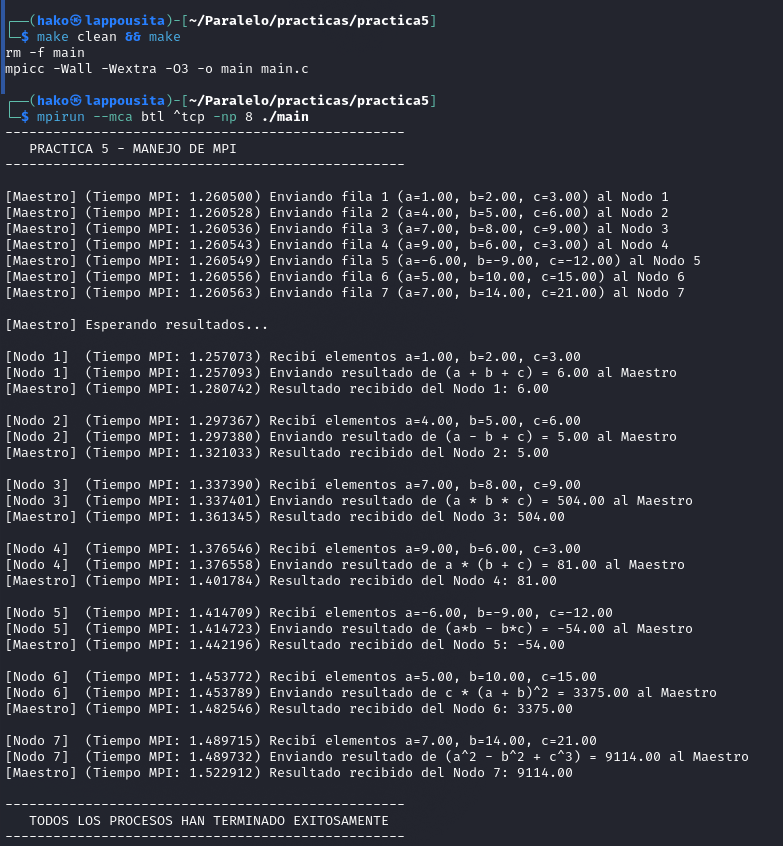
\includegraphics[width=0.9\textwidth]{imagenes/Hako/salida_mpi.png}
\caption{Resultados obtenidos tras la ejecución del programa con MPI. Fuente: Elaboración propia.}
\label{fig:salida_mpi}
\end{figure}



\begin{table}[htbp]
\centering
\caption{Asignación de operaciones y resultados por proceso. Fuente: Elaboración propia.}
\label{tab:operaciones}
\begin{tabular}{|c|c|c|c|}
\hline
\textbf{Nodo} & \textbf{Valores (a, b, c)} & \textbf{Operación Matemática} & \textbf{Resultado Final} \\
\hline
1 & 1.0, 2.0, 3.0 & $a + b + c$ & 6.00 \\
2 & 4.0, 5.0, 6.0 & $a - b + c$ & 5.00 \\
3 & 7.0, 8.0, 9.0 & $a * b * c$ & 504.00 \\
4 & 9.0, 6.0, 3.0 & $a * (b + c)$ & 81.00 \\
5 & -6.0, -9.0, -12.0 & $a * b - b * c$ & -54.00 \\
6 & 5.0, 10.0, 15.0 & $c * (a + b)^2$ & 3375.00 \\
7 & 7.0, 14.0, 21.0 & $a^2 - b^2 + c^3$ & 9114.00 \\
\hline
\end{tabular}
\end{table}

A través del análisis de estos resultados, se valida rotundamente la efectividad de la técnica de paralelización con memoria distribuida en el contexto de la práctica. Asimismo, este bloque final comprueba por completo el alto rendimiento alcanzado al delegar cálculos heterogéneos y dispersos transversalmente sobre un subsistema comunicante que orquesta ordenadamente su diseminación, eliminando posibles estrangulamientos y tiempos muertos de resolución en secuencias ordinarias.


